\section{Background and Related Work}

As mentioned in an earlier section, machine learning has numerous applications
throughout various fields.  Our line of work draws inspiration from 
several areas of research, including the classification of game outcomes and 
prediction of game statistics.  

\textbf{Machine Learning. }
Machine learning is an area in computer science that studies the construction of 
algorithms that can learn from and make predictions on data \cite{5_wikipedia_2015}.  
Relevant machine learning techniques include Principal Component Analysis (PCA), 
sparse coding, support vector machine, and random forests.  PCA is a technique 
commonly used for dimension reduction, which helps with identifying better features 
for a classification or regression task. Sparse coding is a way to automatically 
create a sparse representation of a given input using a set of identified feature 
patterns.  Support vector machines are supervised learning models that analyze and 
recognize patterns, and they can be used as a linear classifier.  Random forests 
are an ensemble learning method for classification that leverages the idea that 
individual classifiers may not be accurate but a group of them may be accurate and 
overcome overfitting.  Our work uses these machine learning techniques to create a 
model to predict the winning team in a League of Legends match.

\textbf{Applications in Games. }
Research by Nicolo Cesa-Bianchi and Gabor Lugosi discuss techniques to aid in 
prediction of games.  Their work concerns prediction with regards to both 
short-term and long-term forecasting.  In chess, the former might be used for 
planning a couple turns 
ahead, whereas the latter may be used for planning a winning strategy.  Their work 
combines previous work on statistical decision theory, game theory, and machine learning 
amongst other related areas.  We employ some of these motivating ideas in developing our
machine learning model.  

\textbf{PageRank. }The algorithm of PageRank emerged from the work of Sergey Brin and Larry 
Page while developing an algorithm to assign values and rankings to web pages \cite{3_page_brin_1998}.  
PageRank highlights several techniques to distinguish useful information 
from junk.  It also details a way to quantify the relationships between different 
useful information.  Since a League of Legends match consists of a team of five versus 
another team of five, the players on each team and their past match histories should 
affect the prediction of which team will win.  

\textbf{LoL Statistics. }
Most League of Legends services provide statistics that are intended to inform about certain statistics about individual champions such as the champion's win rates, play-rate, etc.  There has been little to no prior work in applying machine learning to create models for prediction or classification tasks.

\begin{figure}[t!]
  \centering
    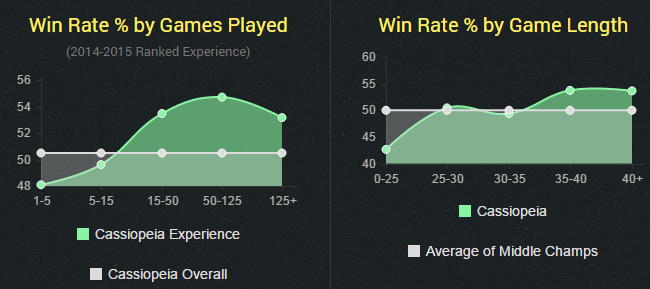
\includegraphics[width=0.5\textwidth]{basic-statistics}
  \caption{Data analysis on games have so far focused on identifying individual statistics, rather than creating models for predicting statistics \cite{6_championgg_2015}. }
  \label{fig:basic-stats}
\end{figure}


\section{Motivation}
The increasing success and applicability of machine learning models in traditional 
sports inspires us to replicate its potential in competitive gaming.  
The competitive scene for League of Legends has been expanding aggressively, 
with many teams hiring analysts to gain deeper insights in the game.  We strongly 
believe that machine learning can play a large role in discovering hidden insights beyond basic stats.  